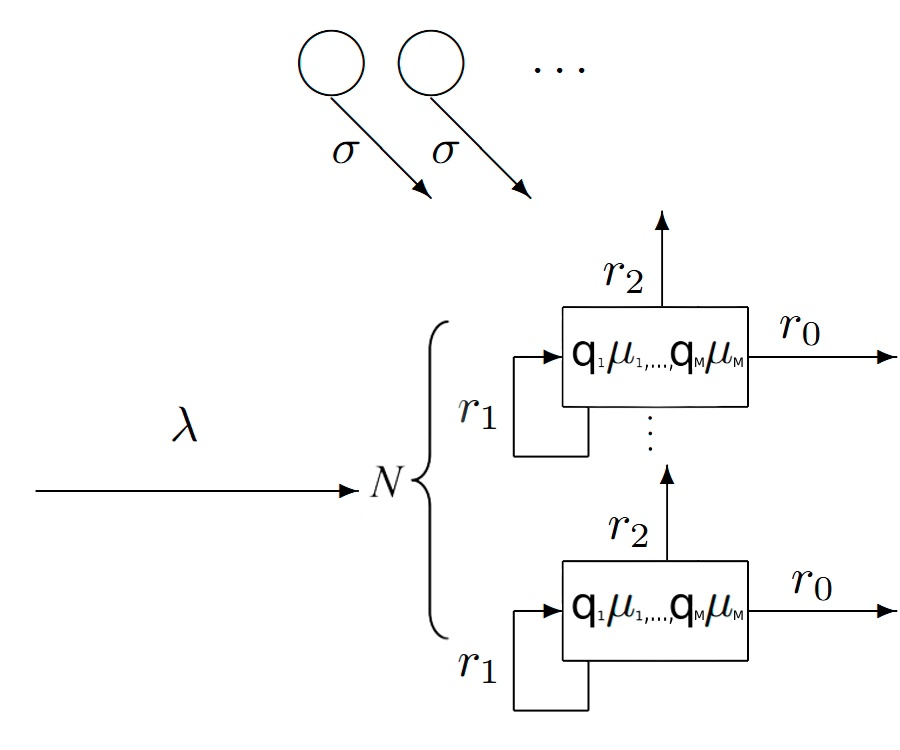
\includegraphics[scale=0.4]{NExecutionMPhase}
\\
Определим пару множеств:
\[\Gt = \{\bold{n} : \sum_{k=1}^{M}n_k < N\}\]
\[\It = \{\bold{n} : \sum_{k=1}^{M}n_k = N\}\]
В данном конкретном случаем определим \(\Jt\) определим как:
\[\Jt = \Gt \cup \It\]

Для упрощения выражений введем индикатор:
\begin{equation*}
    \En =
    \begin{cases}
        1, &{\bold{n} \in \Gt }\\
        0, &{\bold{n} \in \It },
    \end{cases}
\end{equation*}
\begin{equation*}
    \overline{\En} = 1 - \En.
\end{equation*}


